\begin{checkit}
This work is based on \cite{Rao_et_al.-2016-ApJ}, and was carried out in collaboration with the other members of the \AS -CZTI group, to whom I express my sincere thanks, especially to Mithun NPS of the Physical Research Laboratory [PRL], Ahmedabad, India. It heavily relied on the inputs of two of the members, Professor Dipankar Bhattacharya of the Inter-University Centre for Astronomy and Astrophysics [IUCAA], Pune, India; and Vikas Chand, erstwhile graduate student of TIFR, Mumbai, India.
\end{checkit}


\section{Introduction}
\label{sec:introduction--localisation}
The Cadmium Zinc Telluride Imager [CZTI] on-board \AS\ uses an array of pixelated detectors and an equal area and equal size Coded Aperture Mask [CAM] for studying objects in the narrow field of view [FOV] of $4.6^{\circ} \times 4.6^{\circ}$ \citep{Bhalerao_et_al.-2017-JApA}. Being a virtually open detector at energies $> 50$ keV, CZTI does have the possibility of detecting transient events lying outside this narrow FOV. That is exactly what happened with the detection of GRB151006A on the very first day of its operation. This GRB was incident from $\sim 60^{\circ}$ from its pointing axis, as deduced from the \s -BAT sky-localisation of this burst. However, for GRBs incident at such large angles to its pointing axis, the CAM is ineffective. The question arose: Can CZTI independently localise such ``off-axis'' bursts  without the help of the CAM? If so, then the sample of GRBs that would be detected only by CZTI could be followed up in real time at smaller frequencies, enabling detection of their optical/radio afterglows.

\section{Localisation of \grb}
\label{sec:localisation--body}


\begin{figure}
\begin{center}
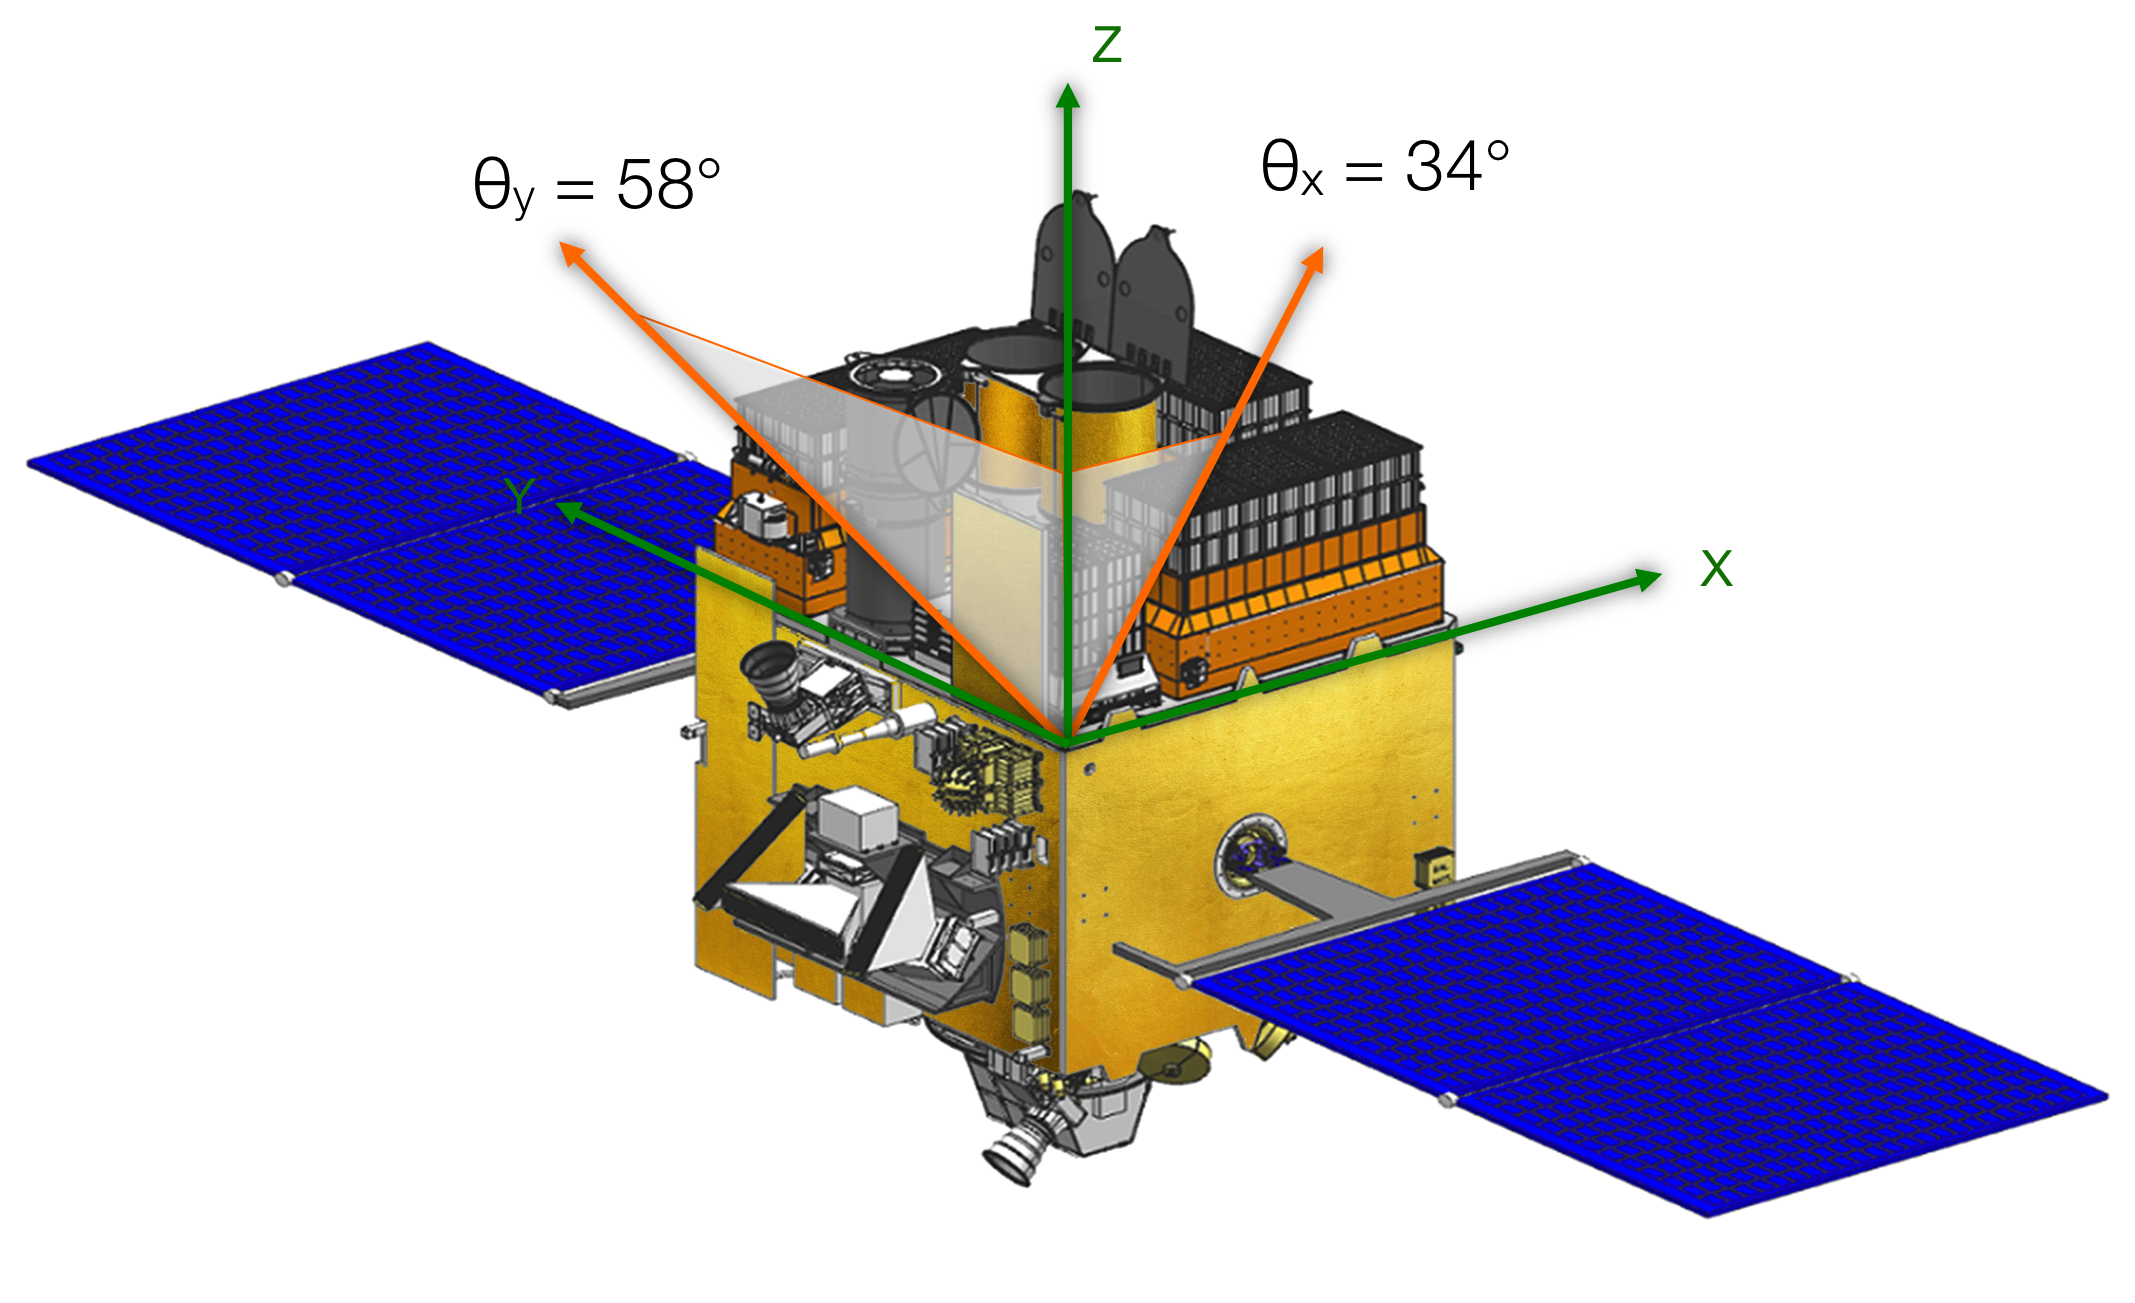
\includegraphics[scale=0.33]{GRB151006A--AstroSat}
\caption[Schematic diagram of the \s\ position of \grb\ with respect to local CZTI co-ordinates]{A schematic picture of \AS\ showing the relative positions of the different instruments, with respect to CZTI. The local coordinate systems of CZTI are defined. The angles $\theta_x$ and $\theta_y$ are measured [in degrees] from the Z-axis in the ZX and ZY planes respectively. The two components of the incident direction of \grb, assuming the sky-position given by \s, are indicated in terms of these angles. Courtesy: \cite{Rao_et_al.-2016-ApJ}.}
\label{fig:GRB151006A--Swift_position}
\end{center}
\end{figure}


In this work, we explored the possibility of using the reasonably accurate position information for individual photons at the detector plane, coupled with the knowledge of mass distribution around the detectors, to localise transient events occurring outside the FOV of CZTI.

Professor Dipankar Bhattacharya [IUCAA, Pune] developed a ray tracing code in the \textsc{fortran} programming language to estimate the effective area of each pixel in the detector plane for an object at a given location in the sky. The mechanical structure given in Figure \ref{fig:CZTI} is represented by $63$ distinct surfaces which are converted into as many cuboids defined by area, thickness, absorbing material, and orientation with respect to the detector surface. For each pixel, the efficiency of transmission through all this material is calculated, along with the detection efficiency of the pixel and geometric projection terms, to give an effective area for a given source direction and energy, for each of the $2^{14} = 16384$ CZTI pixels.

Vikas Chand [erstwhile TIFR, Mumbai] used this off-axis spectral response to generate the spectrum for this GRB for the entire duration of its emission, $\sim 90$ s. The background subtraction was done using pre-burst and post-burst intervals of $90$ s and $200$ s respectively. He then obtained the best-fit parameters of the Band model \citep{Band_et_al.-1993-ApJ}, which fit the spectrum reasonably well.

\begin{figure}
\begin{center}
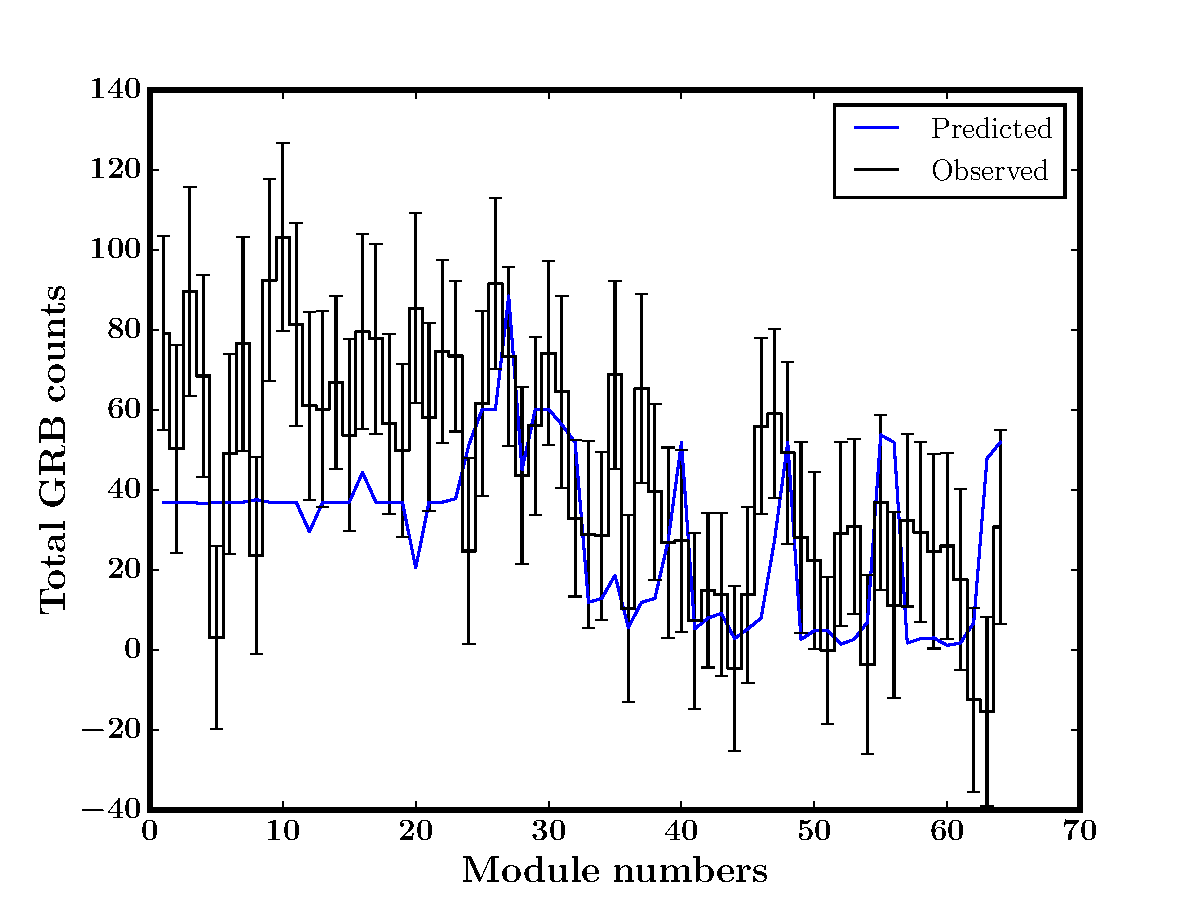
\includegraphics[scale=0.46]{GRB151006A--comparison}
\caption[Comparison between predicted and observed counts of \grb\ versus CZTI modules]{The predicted and observed counts for \grb, corresponding to the $64$ modules, indexed from $0$ to $63$ [according to CZT conventions], for the \s\ position of this GRB [see Figure \ref{fig:GRB151006A--Swift_position}]. The errors on the observed counts assumes statistical [Poisson] errors. Each of the modules is blocked by the instrument materials in a different way, and this is modelled by the ray-tracing code. An overall agreement is seen between the two curves.}
\label{fig:GRB151006A--comparison}
\end{center}
\end{figure}

Using the ray-tracing code, I calculated the pixel-wise efficiency for energies in steps of $5$ keV, for any given angle, expressed in local co-ordinates $\{ \theta_x$, $\theta_y \}$, see Figure \ref{fig:GRB151006A--Swift_position}. This information was then convolved with the spectral model fit to predict the pixel-wise efficiency for this GRB. Since the information in $2^{14}$ pixels is too large and hence the information in each pixel limited below the thresholds of Poisson statistics, the efficiency of all the pixels of a given module were summed, assuming that these pixels are independent of each other. This gave the module-wise counts for any given input angle $\{ \theta_x$, $\theta_y \}$, called the `predicted' counts for that angle.

The `observed' counts in each CZT Module [$64$ in number, indexed from $0$ to $63$ according to CZTI conventions] refers to the number of photons registered in that module for the same time-interval used in the spectral analysis, obtained from the data for this particular GRB, as well as the same pre- and post- burst intervals were chosen to do the background subtraction. A comparison of the predicted and observed counts for the \s\ position of this GRB [see Figure \ref{fig:GRB151006A--Swift_position}] is shown in Figure \ref{fig:GRB151006A--comparison}, and a reasonable agreement is seen.

\begin{figure}
\begin{center}
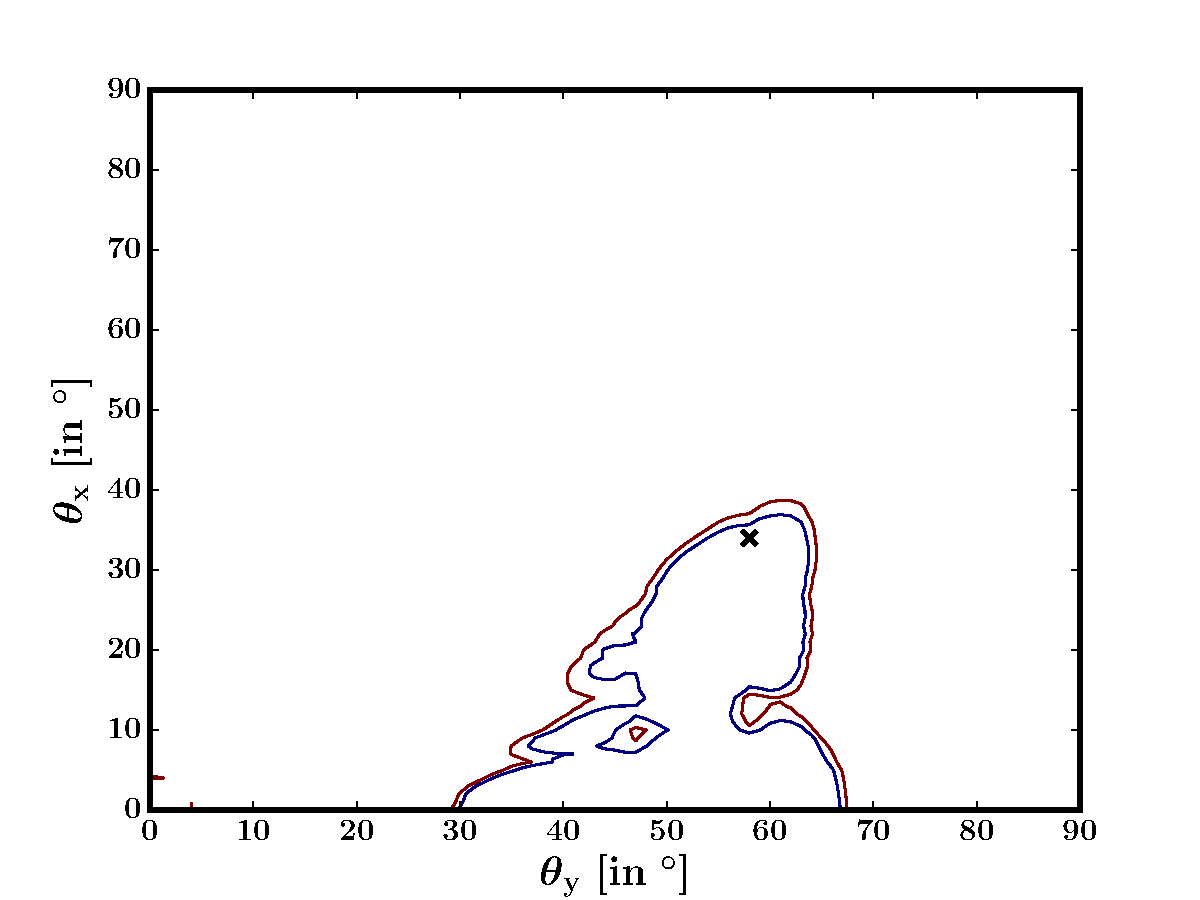
\includegraphics[scale=0.34]{GRB151006A--contours}
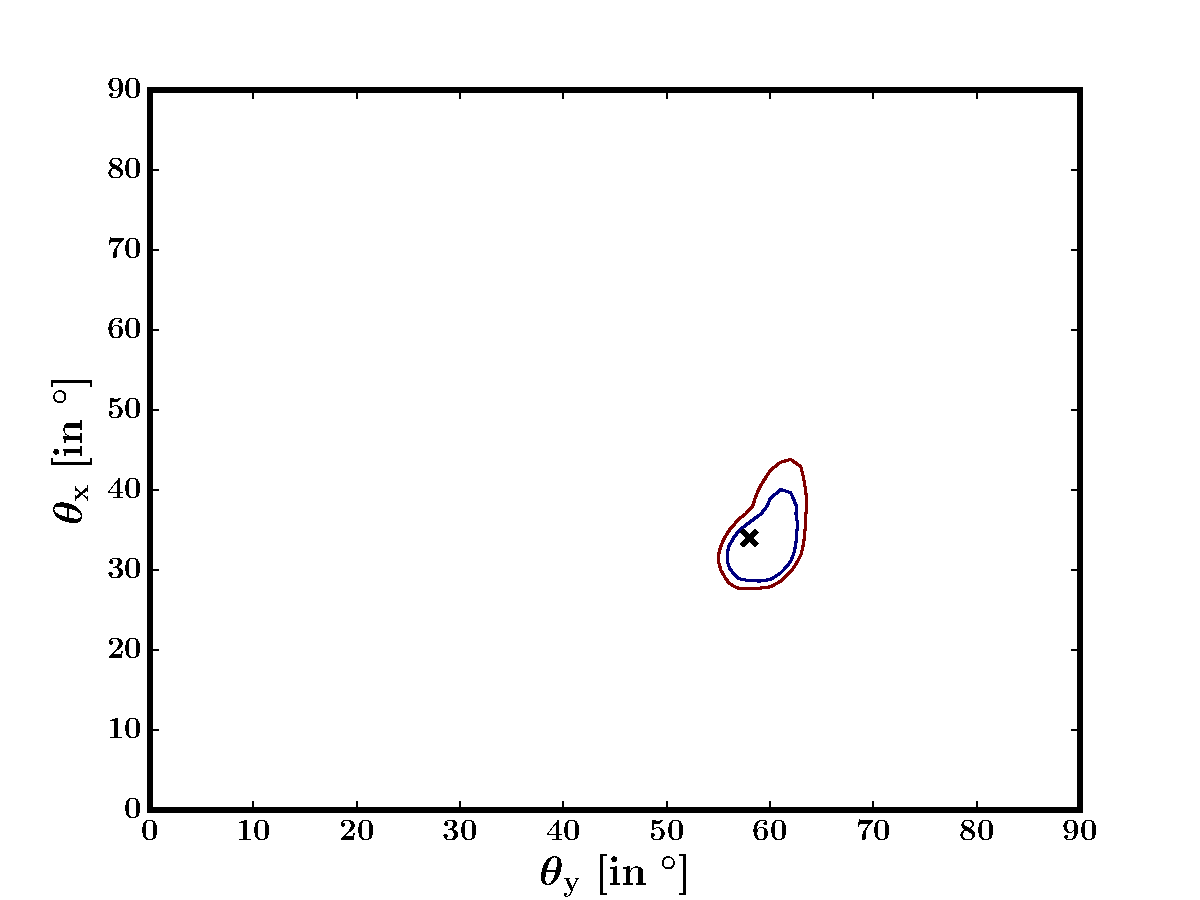
\includegraphics[scale=0.34]{GRB151006A--contours_sim}
\caption[Localisation capabilities of \AS -CZTI: theory and practice]{\eL: Contour plot of the $\chi^2$ between the observed and predicted counts, assuming statistical [Gaussian] errors. The predicted counts are generated for various incident angles, given in the local co-ordinates. The position of \grb\ is marked with a [black-] cross. The blue and brown $\chi^2$ contours correspond to $90 \%$ and $99 \%$ confidence levels, respectively. \eR: The $\chi^2$ contours [colours corresponding to same confidence levels] for a simulated burst of the same fluence, with $1 \sigma$ statistical [Poisson] errors added by hand. Comparison with the contours obtained from the data [left] implies that the assumption of statistical errors on the data is either incorrect or incomplete or both. That is, there is uncharacterised, systematic noise in the data.}
\label{fig:GRB151006A--contours}
\end{center}
\end{figure}

To test the localisation capabilities of CZTI, I simulated the instrument response in a grid of $\{ \theta_x$, $\theta_y \}$ coordinates, in units of $1^{\circ}$ in both $\theta_x$ and $\theta_y$, and convolved it with the spectral fit obtained for this GRB. On comparison with the observed values, the $\chi^2$ as a function of local $\{ \theta_x$, $\theta_y \}$ coordinates was obtained, shown in Figure \ref{fig:GRB151006A--contours}, \eL. It is seen that CZTI could have localised this GRB with an uncertainty of $\sim 10^{\circ}$.

In order to estimate the contribution of statistical errors to the data, I repeated the exercise by comparing simulated detector-wise counts for the $\{ \theta_x$, $\theta_y \}$ grid, with simulated counts for the true location of \grb\ [see Figure \ref{fig:GRB151006A--Swift_position}] and $1 \sigma$ statistical [Poisson] errors added by hand. The confidence contours obtained from this exercise are given in Figure \ref{fig:GRB151006A--contours}, \eR. It is seen that CZTI can localise GRBs of a fluence equal to that of \grb\ with an accuracy of a few degrees, and hence brighter GRBs to even sub-degrees accuracy.

The difference between this idealised case and real data may arise from three primary effects: (a) non-Poissonian errors in the data due to Cosmic Ray interactions; (b) effect of scattering in the detector material; and (c) effects of un-modelled absorption in other parts of the spacecraft. Amongst these, (b) and (c) can be tackled by generating a full mass-model of the entire \AS\ satellite. This means including all the components of the satellite and the relevant masses and the scattering surfaces, and simulating the transmission through as well as scattering from these surfaces. This project was implemented for other GRBs by using the \textsc{geant-4} software \citep{Bhalerao_et_al.-2017-ApJ-A_Tale_of_Two_Transients}, and is currently being integrated into the localisation scheme by new members of the CZTI collaboration. On the other hand, (a) was later studied by myself, and will be extensively discussed in Chapter \ref{chap:noise}.

\section{Conclusions}
\label{sec:conlusions--localisation}
In collaboration with other members of the \AS -CZTI group, it was demonstrated that CZTI is capable of localising \grb\ up to tens of square degrees. This was done by tracing the photons paths through the CZTI surfaces. However, mock data generated from simulations showed that the same GRB should have been localised up to a few degrees if the noise in the data was indeed statistical. The results of a careful investigation of the noise in CZTI data are detailed in Chapter \ref{chap:noise}. Other reasons for the discrepancy could be unaccounted scattering in the CZTI surfaces, or scattering from other payloads on-board \AS. This aspect of the work was expanded upon later by other members of the collaboration.